
\documentclass{beamer}

\mode<presentation> {

% The Beamer class comes with a number of default slide themes
% which change the colors and layouts of slides. Below this is a list
% of all the themes, uncomment each in turn to see what they look like.

%\usetheme{default} % +
%\usetheme{AnnArbor}
%\usetheme{Antibes}
%\usetheme{Bergen}
%\usetheme{Berkeley} % +
%\usetheme{Berlin}
%\usetheme{Boadilla} % +
%\usetheme{CambridgeUS}
%\usetheme{Copenhagen}
%\usetheme{Darmstadt}
%\usetheme{Dresden} 
%\usetheme{Frankfurt} % +
%\usetheme{Goettingen}
%\usetheme{Hannover}
%\usetheme{Ilmenau}
%\usetheme{JuanLesPins}
%\usetheme{Luebeck}
%\usetheme{Madrid} % +
%\usetheme{Malmoe}
%\usetheme{Marburg}
%\usetheme{Montpellier}
%\usetheme{PaloAlto}
%\usetheme{Pittsburgh}
%\usetheme{Rochester}
\usetheme{Singapore} % +
%\usetheme{Szeged}
%\usetheme{Warsaw}

% As well as themes, the Beamer class has a number of color themes
% for any slide theme. Uncomment each of these in turn to see how it
% changes the colors of your current slide theme.

%\usecolortheme{albatross}
%\usecolortheme{beaver}
%\usecolortheme{beetle}
%\usecolortheme{crane}
%\usecolortheme{dolphin}
%\usecolortheme{dove}
%\usecolortheme{fly}
%\usecolortheme{lily}
%\usecolortheme{orchid}
%\usecolortheme{rose}
%\usecolortheme{seagull}
%\usecolortheme{seahorse}
%\usecolortheme{whale}
%\usecolortheme{wolverine}

%\setbeamertemplate{footline} % To remove the footer line in all slides uncomment this line
%\setbeamertemplate{footline}[page number] % To replace the footer line in all slides with a simple slide count uncomment this line

%\setbeamertemplate{navigation symbols}{} % To remove the navigation symbols from the bottom of all slides uncomment this line
}


%\logo{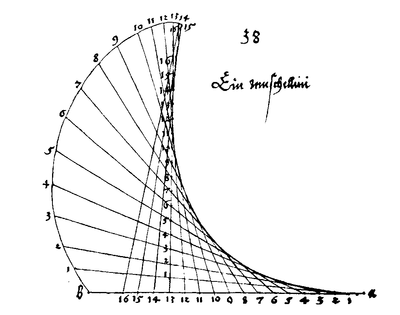
\includegraphics[height=1cm]{./images/logo.png}}


\usepackage{graphicx} % Allows including images
\usepackage{booktabs} % Allows the use of \toprule, \midrule and \bottomrule in tables
\usepackage{caption}
\usepackage{subcaption}
\usepackage{array}
%\usepackage{tcolorbox}
%\usepackage{enumitem}

%----------------------------------------------------------------------------------------
%   TITLE PAGE
%----------------------------------------------------------------------------------------

\title[Epidemics Wokrshop]{G-CSC Epidemics\newline Disease modelling via SEIRD}

\author{\textcolor{blue}{Yannick Rosam\\}}
\institute[G-CSC] % Your institution as it will appear on the bottom of every slide, may be shorthand to save space
{
Goethe - Center for Scientific Computing \\ % Your institution for the title page
\medskip
%\textit{john@smith.com} % Your email address
}
%\date{\today} % Date, can be changed to a custom date
\begin{document}
\begin{frame}
\frametitle{The Horror of Today}
        // mass given in grams\\
        // volume given in liter($dm^3$)\\
        // returns density in $kg/m^3$\\
        double calculate\_density(double mass, double volume)\\
        \{\\
        \ \ \ \ // todo implement conversion of mass to kg\\
        \ \ \ \ // todo implement conversion volume to to $m^{3}$\\
        \ \ \ \ return density;\\
        \}
\end{frame}

\begin{frame}
\frametitle{Formulating the Problem}
\begin{enumerate}
\item There are many different kinds of units we use daily, and they come in a vast amount of forms and sizes.
\item Calculation with different kinds of them and the conversion involving can be challenging at times...
\item ...especially working in a scientific environment
\end{enumerate}
\end{frame}
\begin{frame}

\frametitle{Idea}
A simple framework that \ldots
\begin{enumerate}[label=\ldots]
\item takes care of these conversions for you,
\item without imparting your coding speed 
\item and also makes code better to understand.
\end{enumerate}

\end{frame}

\begin{frame}
\frametitle{Solution and Implementation}

- Using custom underscore operator, to write the units directly in the formula like one would on paper.

- So you can write the formula for physical force e.g. just like x\_kg * 1\_m / 1\_s2, where x would be a variable of type float, double, integer or any alike number datatype.

- or if you want to drop the 1\_ Parts, where you dont need the, you could just create an intermediate variable like double kg = 1\_kg and just use a standalone kg.
\end{frame}

\begin{frame}
\frametitle{How we would do it now}
    
 
\end{frame}


\begin{frame}{Possible Variants of one specific Formula}
    

Die Teilchenzahl N einer 3-millimolaren (3 mM) Lösung von Rohrzucker in Wasser bei einem Lösungsvolumen $V = 2$ Kubikzentimeter, wobei $N_{A}$ (Avogadro-Konstante) die Anzahl der Teilchen pro Mol angibt, beträgt:


$ c C_{12} H_{22} O_{11} * V * N_{A} =0.003\frac{mol}{dm^{3}} \cdot 0.002 dm^{3} \cdot 6.022 \cdot 10^{23}mol^{-1} $


In code that would be something like:
\[
\begin{array}{c}
(0.003\_mol / 1\_dm^{3}) * 0.002\_dm^{3} * 6.022 * 10^{23}\_mol^{-1}\\
&Or\\
&3\_mmol\_per\_dm^{-3} * 2\_cm^{3} * 6.022 * 10^{23}\_mol
\end{array}
\]


Or just 
\hyperlink{https://www.chemie.de/lexikon/images/math/a/8/5/a859b3abf3767634b37de76f7c9d7529.png}

 
All these and more would be possible with our cppunits library. 
Furthermore.you will soon be able to implement your own custom units with the click of  a button.
This can be done without understanding or even reading the underlying codebase, through a simple formula2code parser system.

\end{frame}

\end{document}
